\documentclass[12pt]{article}
\usepackage{fancyhdr}
\usepackage{amsmath,amsfonts,enumerate}
\usepackage{color,graphicx}
\usepackage{tikz}
\usepackage{pgfplots}
\usepackage{listings}
\usepackage{algorithm}
\usepackage{algorithmic}
\usetikzlibrary{arrows,positioning,shapes,calc,matrix}
\pagestyle{fancy}
%%%%%%%%%%%%%%%%%%%%%%%%%%%%%%%%%%%%%%%%%%%%%%%%%
% Course customization based on university sources
%%%%%%%%%%%%%%%%%%%%%%%%%%%%%%%%%%%%%%%%%%%%%%%%%
\newcommand{\masunitnumber}{CENG 403}
\newcommand{\examdate}{January 2025}
\newcommand{\academicyear}{2024-2025}
\newcommand{\semester}{I}
\newcommand{\coursename}{Deep Learning - CNN Architecture Design \& Transfer Learning (University Sources)}
\newcommand{\numberofhours}{3}
%%%%%%%%%%%%%%%%%%%%%%%%%%%%%%%%%%%%%%%%%%%%%%%%%
% CUSTOM SPACING COMMANDS FOR ANSWER SPACES
%%%%%%%%%%%%%%%%%%%%%%%%%%%%%%%%%%%%%%%%%%%%%%%%%
\newcommand{\answerspace}[1]{\vspace{#1}}
\newcommand{\questionspace}{\vspace{3cm}}        
\newcommand{\subquestionspace}{\vspace{2.5cm}}   
\newcommand{\shortanswer}{\vspace{2cm}}          
\newcommand{\mediumanswer}{\vspace{3cm}}         
\newcommand{\longanswer}{\vspace{4cm}}           
\newcommand{\journalspace}{\vspace{4.5cm}}       
\newcommand{\codespace}{\vspace{5cm}}            
%%%%%%%%%%%%%%%%%%%%%%%%%%%%%%%%%%%%%%%%%%%%%%%%%
% Header setup
%%%%%%%%%%%%%%%%%%%%%%%%%%%%%%%%%%%%%%%%%%%%%%%%%
\lhead{}
\rhead{}
\chead{{\bf MIDDLE EAST TECHNICAL UNIVERSITY}}
\lfoot{}
\rfoot{}
\cfoot{}
\begin{document}
\setlength{\headsep}{5truemm}
\setlength{\headheight}{14.5truemm}
\setlength{\voffset}{-0.45truein}
\renewcommand{\headrulewidth}{0.0pt}
\begin{center}
SEMESTER \semester\ EXAMINATION \academicyear
\end{center}
\begin{center}
{\bf \masunitnumber\ -- \coursename}
\end{center}
\vspace{20truemm}
\noindent \examdate\hspace{45truemm} TIME ALLOWED: \numberofhours\ HOURS
\vspace{19truemm}
\hrule
\vspace{19truemm}
\noindent\underline{INSTRUCTIONS TO CANDIDATES}
\vspace{8truemm}
%%%%%%%%%%%%%%%%%%%%%%%%%%%%%%%%%%%%%%%%%%%%%%%%%%%%%%
% Instructions based on university standards
%%%%%%%%%%%%%%%%%%%%%%%%%%%%%%%%%%%%%%%%%%%%%%%%%%%%%%
\begin{enumerate}
\item This examination paper contains {\bf SEVEN (7)} questions and comprises 
{\bf TEN (10)} printed pages.
\item Answer all questions. 
The marks for each question are indicated at the beginning of each question.
\item Answer each question beginning on a {\bf FRESH} page of the answer book.
\item This {\bf IS NOT an OPEN BOOK} exam.
\item Show all mathematical derivations clearly with proper notation.
\item For architectural diagrams, draw clear and labeled components.
\item Calculate all requested parameters and show intermediate steps.
\item Explain computational complexity where requested.
\end{enumerate}
%%%%%%%%%%%%%%%%%%%%%%%%%%%%%%%%%%%%%%%%%%%%%%%%%
% New page for questions
%%%%%%%%%%%%%%%%%%%%%%%%%%%%%%%%%%%%%%%%%%%%%%%%%
\newpage
\lhead{}
\rhead{\masunitnumber}
\chead{}
\lfoot{}
\cfoot{\thepage}
\rfoot{}
\setlength{\footskip}{45pt}
%%%%%%%%%%%%%%%%%%%%%%%%%%%%%%%%%%%%%%%%%%%%%%%%%%
% EXAM QUESTIONS BASED ON UNIVERSITY SOURCES
%%%%%%%%%%%%%%%%%%%%%%%%%%%%%%%%%%%%%%%%%%%%%%%%%%

\paragraph{Question 1. Position-Sensitive Convolution Mathematical Analysis}{{\hfill (25 marks)}}\\
Based on Stanford CS231n and university computer vision course materials.

\begin{enumerate}[(a)]
    \item Formulate position-sensitive convolution mathematically. Given input $X \in \mathbb{R}^{H \times W \times C}$, derive the augmented input formulation: \hfill (10 marks)
    \begin{itemize}
        \item Show $X_{aug}(i,j) = [X(i,j), \frac{i}{H}, \frac{j}{W}]$ where coordinates are normalized to [0,1]
        \item Explain why vanilla convolution fails for position estimation tasks
        \item Calculate the increased computational cost: memory and FLOPs for coordinate channels
    \end{itemize}
    
    \journalspace
    
    \item Analyze the mathematical foundation of pooling invariances. For max pooling with receptive field $R$ and stride $s$: \hfill (10 marks)
    \begin{itemize}
        \item Derive translation invariance: if $X'(i,j) = X(i+\delta, j+\delta)$ where $|\delta| < s$, show when $\text{MaxPool}(X') = \text{MaxPool}(X)$
        \item Calculate the exact translation tolerance for different pooling configurations
        \item Compare mathematical properties of max pooling vs. average pooling for invariance
    \end{itemize}
    
    \mediumanswer
    
    \item Design an experimental validation for position-sensitive convolution effectiveness: \hfill (5 marks)
    \begin{itemize}
        \item Propose synthetic datasets for controlled position estimation evaluation
        \item Define quantitative metrics for position accuracy assessment
        \item Statistical significance testing for performance comparison
    \end{itemize}
    
    \shortanswer
\end{enumerate}

\newpage
\paragraph{Question 2. Global Average Pooling vs. Fully Connected Layers}{{\hfill (28 marks)}}\\
Based on MIT 6.034 and university machine learning course materials.

\begin{enumerate}[(a)]
    \item Analyze the parameter explosion problem in fully connected layers. For a CNN with final feature map of size $H \times W \times C$ and $N$ output classes: \hfill (12 marks)
    \begin{itemize}
        \item Calculate exact parameter count for FC approach: $(H \times W \times C) \times N + N$
        \item Show GAP parameter count: $C \times N + N$
        \item For AlexNet (6×6×256 → 4096 → 4096 → 1000), compute parameter reduction percentage
        \item Analyze memory footprint implications for training and inference
    \end{itemize}
    
    \journalspace
    
    \item Prove the mathematical equivalence between GAP and specialized channel learning: \hfill (10 marks)
    \begin{itemize}
        \item Given feature map $F_k(x,y)$ for channel $k$, show GAP output: $g_k = \frac{1}{HW}\sum_{x,y} F_k(x,y)$
        \item Derive how network learns to optimize: $\max_{F_k} \sum_k w_{k,c} \cdot g_k$ for class $c$
        \item Explain why this forces $F_k$ to become confidence maps for specific objects
        \item Mathematical justification for why "one fully connected layer is sufficient"
    \end{itemize}
    
    \mediumanswer
    
    \item Evaluate GAP limitations and failure cases: \hfill (6 marks)
    \begin{itemize}
        \item When does the assumption $C \approx N$ (channels ≈ classes) break down?
        \item Mathematical analysis of information loss compared to FC layers
        \item Propose hybrid architectures combining GAP benefits with FC expressiveness
    \end{itemize}
    
    \shortanswer
\end{enumerate}

\newpage
\paragraph{Question 3. Fully Convolutional Networks Theory and Implementation}{{\hfill (22 marks)}}\\
Based on UC Berkeley computer vision courses and research literature.

\begin{enumerate}[(a)]
    \item Derive the mathematical transformation from FC to convolutional layers: \hfill (10 marks)
    \begin{itemize}
        \item For FC layer with weight matrix $W \in \mathbb{R}^{M \times N}$ and input $x \in \mathbb{R}^N$
        \item Show equivalence: $y = Wx$ ↔ $y = \text{Conv}(x, W_{reshaped})$ with appropriate kernel size
        \item Calculate output dimensions: input $H' \times W'$ → output $(H'-H+1) \times (W'-W+1)$ prediction maps
        \item Prove that this enables processing of arbitrary input sizes
    \end{itemize}
    
    \journalspace
    
    \item Analyze computational efficiency of fully convolutional approach: \hfill (8 marks)
    \begin{itemize}
        \item Compare computational cost: multiple forward passes vs. single FCN pass
        \item Calculate speedup factor for image classification on different resolution inputs
        \item Memory usage analysis: activation map storage vs. multiple network copies
    \end{itemize}
    
    \mediumanswer
    
    \item Design FCN applications beyond image classification: \hfill (4 marks)
    \begin{itemize}
        \item Semantic segmentation: pixel-level classification formulation
        \item Object detection: sliding window with efficiency gains
        \item Heatmap generation for localization tasks
    \end{itemize}
    
    \shortanswer
\end{enumerate}

\newpage
\paragraph{Question 4. CNN Architecture Design Principles and Empirical Analysis}{{\hfill (30 marks)}}\\
Based on comprehensive university deep learning course materials and research findings.

\begin{enumerate}[(a)]
    \item Analyze the empirical study on filter size, depth, and width trade-offs: \hfill (15 marks)
    \begin{itemize}
        \item Mathematical formulation: for fixed computational budget $B$, analyze trade-off between depth $D$, width $W$, and filter size $F$
        \item Explain why "deeper networks with smaller filters provided better results"
        \item Calculate effective receptive field: for $L$ layers with filter size $F$, show receptive field = $1 + L(F-1)$
        \item Prove that depth provides exponential expressiveness increase while maintaining linear parameter growth
    \end{itemize}
    
    \begin{center}
    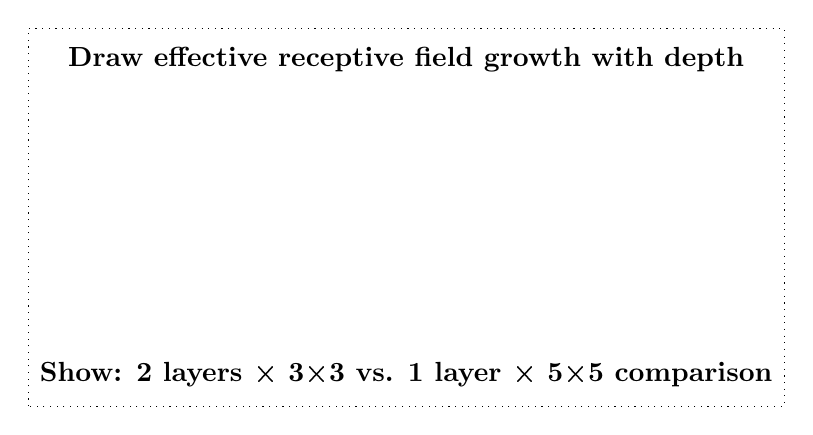
\begin{tikzpicture}[scale=0.8]
        % Space for receptive field calculation diagram
        \draw[dotted] (0,0) rectangle (12,6);
        \node at (6,5.5) {\textbf{Draw effective receptive field growth with depth}};
        \node at (6,0.5) {\textbf{Show: 2 layers × 3×3 vs. 1 layer × 5×5 comparison}};
    \end{tikzpicture}
    \end{center}
    
    \shortanswer
    
    \item Design memory-efficient CNN architectures using the "reduce dimensionality early" principle: \hfill (10 marks)
    \begin{itemize}
        \item Calculate memory footprint: for input $224 \times 224 \times 3$, compare memory usage with stride=1 vs. stride=4 in first layer
        \item Justify why "information is redundant in earlier layers" from information theory perspective
        \item Design optimal stride schedule for 8-layer network balancing memory and performance
    \end{itemize}
    
    \mediumanswer
    
    \item Evaluate architectural design patterns across successful CNN families: \hfill (5 marks)
    \begin{itemize}
        \item Progressive resolution reduction: mathematical analysis of optimal reduction schedule
        \item Channel expansion strategies: when and why to increase feature map depth
        \item Computational vs. accuracy trade-offs in mobile architectures
    \end{itemize}
    
    \shortanswer
\end{enumerate}

\newpage
\paragraph{Question 5. Transfer Learning Mathematical Framework and Analysis}{{\hfill (25 marks)}}\\
Based on domain adaptation theory and university machine learning courses.

\begin{enumerate}[(a)]
    \item Formalize the four transfer learning scenarios using mathematical notation: \hfill (12 marks)
    
    Let source domain $\mathcal{D}_s = \{X_s, P(X_s)\}$, target domain $\mathcal{D}_t = \{X_t, P(X_t)\}$, source task $\mathcal{T}_s = \{Y_s, f_s(\cdot)\}$, target task $\mathcal{T}_t = \{Y_t, f_t(\cdot)\}$:
    
    \begin{itemize}
        \item Scenario 1: $\mathcal{T}_s \approx \mathcal{T}_t$, $|D_t| < \text{threshold}$ → Freeze weights $\theta_{1:L-1}$, train only $\theta_L$
        \item Scenario 2: $\mathcal{T}_s \approx \mathcal{T}_t$, $|D_t| > \text{threshold}$ → Fine-tune all $\theta_{1:L}$ with small learning rate
        \item Scenario 3: $\mathcal{T}_s \not\approx \mathcal{T}_t$, $|D_t| < \text{threshold}$ → Use $\theta_{1:k}$, retrain $\theta_{k+1:L}$
        \item Scenario 4: $\mathcal{T}_s \not\approx \mathcal{T}_t$, $|D_t| > \text{threshold}$ → Fine-tune all layers
    \end{itemize}
    
    \journalspace
    
    \item Analyze the theoretical foundation of layer transferability: \hfill (8 marks)
    \begin{itemize}
        \item Prove why early layers learn "generic, problem-independent" features using information theory
        \item Mathematical justification for "later parts are problem-dependent"
        \item Quantify transferability: define similarity metrics between feature representations
    \end{itemize}
    
    \mediumanswer
    
    \item Design optimal learning rate schedules for transfer learning: \hfill (5 marks)
    \begin{itemize}
        \item Derive layer-wise learning rate adaptation: $\eta_l = \eta_0 \cdot \alpha^{L-l}$ where $\alpha < 1$
        \item Explain why "you can easily disrupt the learned weights" with high learning rates
        \item Propose adaptive learning rate methods based on layer depth and similarity metrics
    \end{itemize}
    
    \shortanswer
\end{enumerate}

\newpage
\paragraph{Question 6. CNN Visualization Techniques Mathematical Framework}{{\hfill (28 marks)}}\\
Based on interpretable AI research and university courses on explainable machine learning.

\begin{enumerate}[(a)]
    \item Implement gradient-based saliency map generation with mathematical rigor: \hfill (12 marks)
    \begin{itemize}
        \item Derive saliency map: $S_i = \left|\frac{\partial f_c(x)}{\partial x_i}\right|$ for class $c$
        \item Linear approximation justification: $f(x + \epsilon) \approx f(x) + \epsilon^T \nabla_x f(x)$
        \item Implementation using backpropagation: chain rule application through network layers
        \item Compare with integrated gradients: $\text{IG}_i = (x_i - x'_i) \times \int_{\alpha=0}^1 \frac{\partial f(x' + \alpha(x-x'))}{\partial x_i} d\alpha$
    \end{itemize}
    
    \journalspace
    
    \item Analyze occlusion-based sensitivity analysis: \hfill (10 marks)
    \begin{itemize}
        \item Formulate occlusion experiment: $\Delta_p = f(x) - f(x \odot M_p)$ where $M_p$ is occlusion mask
        \item Statistical significance testing for determining important regions
        \item Design optimal occlusion window sizes and stride patterns
        \item Distinguish between network memorization vs. proper feature learning
    \end{itemize}
    
    \mediumanswer
    
    \item Evaluate visualization quality using quantitative metrics: \hfill (6 marks)
    \begin{itemize}
        \item Localization accuracy: IoU with ground truth bounding boxes
        \item Fidelity metrics: correlation between saliency scores and true importance
        \item Computational efficiency: runtime complexity analysis for different methods
    \end{itemize}
    
    \shortanswer
\end{enumerate}

\newpage
\paragraph{Question 7. Advanced CNN Topics Integration and Analysis}{{\hfill (22 marks)}}\\
Based on comprehensive university deep learning curricula and research literature.

\begin{enumerate}[(a)]
    \item Design a comprehensive CNN architecture combining all discussed techniques: \hfill (12 marks)
    \begin{itemize}
        \item Architecture specification: incorporate position-sensitive conv, GAP, transfer learning capability
        \item Mathematical analysis: parameter count, memory footprint, computational complexity
        \item Training strategy: multi-stage training with different learning rates for different components
        \item Evaluation protocol: metrics for both accuracy and interpretability
    \end{itemize}
    
    \begin{center}
    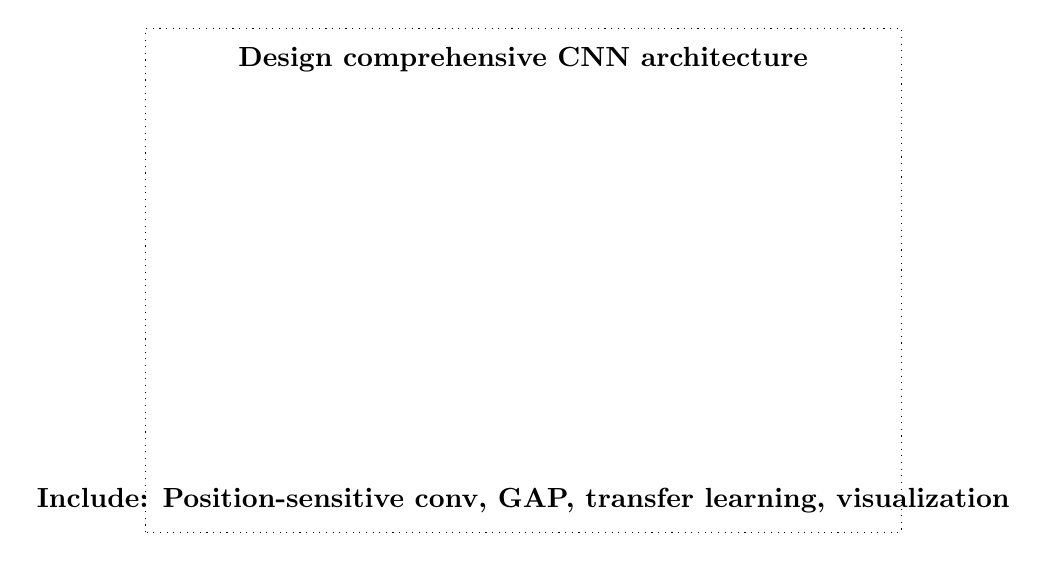
\begin{tikzpicture}[scale=0.8]
        % Space for comprehensive architecture design
        \draw[dotted] (0,0) rectangle (12,8);
        \node at (6,7.5) {\textbf{Design comprehensive CNN architecture}};
        \node at (6,0.5) {\textbf{Include: Position-sensitive conv, GAP, transfer learning, visualization}};
    \end{tikzpicture}
    \end{center}
    
    \shortanswer
    
    \item Analyze failure modes and limitations of discussed techniques: \hfill (10 marks)
    \begin{itemize}
        \item Position-sensitive convolution: computational overhead and when it's unnecessary
        \item GAP limitations: information bottleneck and class imbalance effects
        \item Transfer learning: negative transfer and domain shift problems
        \item Visualization techniques: interpretation biases and validation challenges
    \end{itemize}
    
    \mediumanswer
\end{enumerate}

\vfill
\begin{center}{\bf END OF PAPER}\end{center>
\end{document}